\documentclass[18pt]{article}
\usepackage[a1paper,margin=1in,landscape]{geometry}
\usepackage{multicol}
\setlength{\columnsep}{1cm}
\usepackage{blindtext}
%\usepackage{tabularx}
\usepackage{booktabs}
\usepackage{tikz}
\usepackage{float}
\usepackage{pgfplots}
\usepackage{pgfplotstable}
% \pgfplotsset{width=\textwidth, compat=newest}
\pgfplotsset{compat=newest}
\usepgfplotslibrary{statistics}
%% new command defs
\newcommand\boxplotbignum{1000000}
\usetikzlibrary{calc}

%%
%%
\begin{document}
\begin{multicols}{3}
[
	\section{Datasets and Basic Properties}
	Real-world datasets and degree distributuion, clustering coefficients, and hopplot.	
]
%\begin{tabularx}{\columnwidth}{@{} l l X @{}} 
\begin{tabular}{@{} llr @{}}
% datasets - https://github.com/briatte/awesome-network-analysis#datasets
	\textbf{Dataset} & \textbf{Details} & \textbf{$n$}\\

\toprule
	PP PDZBase	& Protein–protein interactions from PDZBase & $212$\\
	College & College Messages (email) & $1899$\\
	Routers 2001 & Route Views AS graphs (1999-2000)	& $6474$\\
	Routers 2006 & Internet AS graph (2006)						& $22963$\\
	Retweet 2012 & Twitter Higgs Boson (Retweet) & $425008$
\end{tabular}

\begin{figure}[H]
  \centering
	\resizebox{\columnwidth}{!}{
		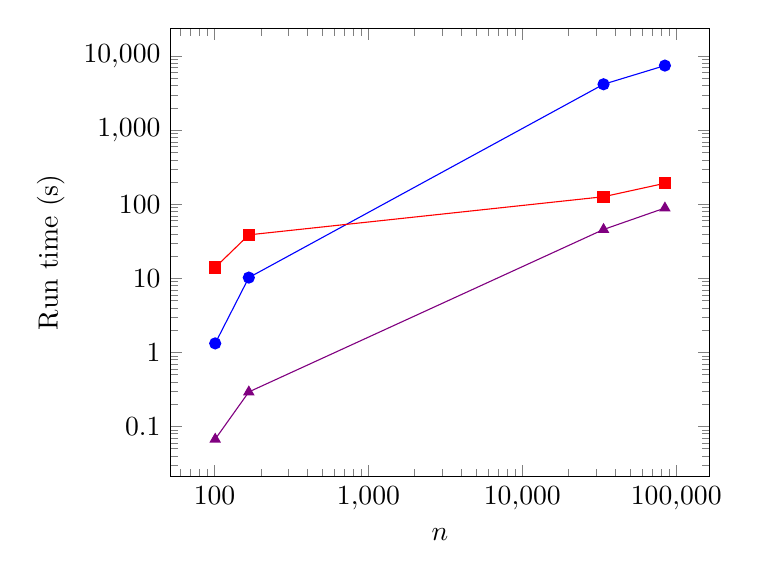
\begin{tikzpicture}
    \begin{loglogaxis}[xlabel=$n$,
			ylabel=Run time (s),
			log ticks with fixed point,]
      % [width=\linewidth,
      %            height=4cm, enlarge y limits=.2,
      %            ytick={1, 2}] % , yticklabels={Wrong, Right}
      %\addplot+ [boxplot={whisker range=\boxplotbignum}] table [y index=0] {figures/data.1.txt};
      % Ignore the miscalculations here
      %\addplot+ [boxplot prepared={draw position=2,
      %                             median=662,
      %                             lower whisker=222,
      %                             upper whisker=1558,
      %                             upper quartile=867,
      %                             lower quartile=478.5}] coordinates {};
	%% 
	%% Runtime for computing k number of graphs as a function of datasets' number of nodes
	%%
  %	EMAIL CORE
  %	RADOSLAW
	%	enron (full)
	%	email-Enron.txt
  %% PHRG
    \addplot[color=blue,mark=*] table [col sep=comma]
			{
      101, 1.32355809212
      167, 10.2496099472
			33696, 4188.344877
      84384, 7487.98321414
      };
    %% CHLU
    \addplot[color=violet,mark=triangle*] table [col sep=comma]
    	{
      101, 0.0673129558563
      167, 0.292577981949
			33696, 45.7626059055
      84384, 89.1664869785
      };

    %% KRON
    \addplot[color=red,mark=square*] table [col sep=comma]
			{
			101, 14.0635240078
      167, 38.7150030136
			33696, 126.776366949
      84384, 192.528311968
			};
    \end{loglogaxis}
\end{tikzpicture}

		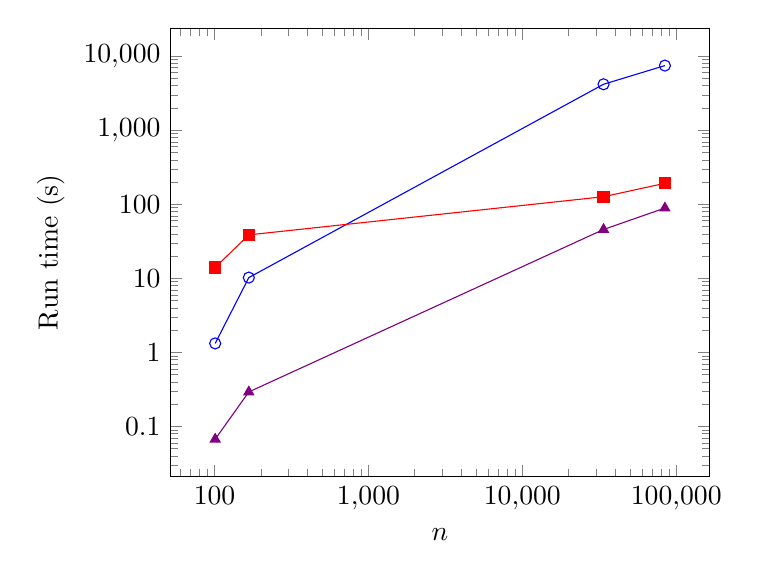
\begin{tikzpicture}
  \begin{loglogaxis}[xlabel=$n$,
			ylabel=Run time (s),
			log ticks with fixed point,
  ]
	%%
	%% Runtime for computing k number of graphs as a function of datasets' number of nodes
  %% Using Rods (stochastic graph generation)
	%%
  %	EMAIL CORE
  %	RADOSLAW
	%	enron (full)
	%	email-Enron.txt
  %% PHRG
  \addplot[color=blue, mark=o] table [col sep=comma]
			{
      101, 1.32355809212
      167, 10.2496099472
			33696, 4188.344877
      84384, 7487.98321414
      };
  %% CHLU
  \addplot[color=violet,mark=triangle*] table [col sep=comma]
    	{
      101, 0.0673129558563
      167, 0.292577981949
			33696, 45.7626059055
      84384, 89.1664869785
      };

  %% KRON
  \addplot[color=red,mark=square*] table [col sep=comma]
		  {
			101, 14.0635240078
      167, 38.7150030136
			33696, 126.776366949
      84384, 192.528311968
			};
    \end{loglogaxis}
\end{tikzpicture}

		\begin{tikzpicture}
\begin{axis} [
  only marks,
  ymode = log,
    xlabel     = Degree ($k$), % label x axis
    ylabel     = Cumulative probability, % label y axis
    axis lines = left, %set the position of the axes
    clip       = false,
    % xmin = 40,  xmax = 105, % set the min and max values of the x-axis
    % ymin = 150, ymax = 200, % set the min and max values of the y-axis
    title= {\Large \textbf{(C)}}
    ]
  % \addplot [only marks] table {Pltdata/ucidata-gama_degCDF.dat};ikey	origCDF	phrgDegCDF
  % \addplot[color=blue,mark=*] table [col sep=tab]
\addplot[color=red, mark=*, opacity=0.5] table [x index=0,y index=1,col sep=tab]{figures/kecdf_radoslaw_email_email_rods_hstars.dat};
\addplot[color=blue,mark=sqaure, opacity=0.5] table [x index=0,y index=2,col sep=tab]{figures/kecdf_radoslaw_email_email_rods_hstars.dat};
\addplot[color=cyan,mark=+,opacity=0.5] table [x index=0,y index=2,col sep=tab]{figures/kecdf_radoslaw_email_email_clgs.dat};
\addplot[color=black,mark=diamond,opacity=0.5] table [x index=0,y index=2,col sep=tab]{figures/kecdf_radoslaw_email_email_kpgs.dat};
% \addplot table[x index=0,y index=2,col sep=tab]
% {figures/kecdf_rados.dat};
% ('email-Eu-core-Dept1_rods.shl', ['rods_hstars', 'clgs', 'kpgs'])
% rods_hstars 10
% ----------------------------------------
% Scaled-Normalized Degree Dist CDF radoslaw_email_email_rods_hstars

%   \addplot[color=red,mark=square*,opacity=0.5] table [col sep=comma]
%   {
% 0.972972972973, 4.44075746485e-21
% 0.973684210526, 1.8802452137e-21
% 0.971428571429, 2.60839605838e-20
% 0.972222222222, 1.06684630059e-20
% 0.974358974359, 8.0939108781e-22
% 0.972222222222, 1.06684630059e-20
% 0.972972972973, 4.44075746485e-21
% 0.974358974359, 8.0939108781e-22
% 0.972222222222, 1.06684630059e-20
% 0.97619047619, 7.09701552086e-23
% };
%
% %kpgs 10
%   \addplot[color=violet,mark=triangle*,opacity=0.5] table [col sep=comma]
% {
% 0.439393939394, 0.000416044895695
% 0.511904761905, 3.38254947171e-05
% 0.378787878788, 0.00367101440595
% 0.424242424242, 0.000739070116185
% 0.393939393939, 0.00141702410322
% 0.454545454545, 0.000229529638995
% 0.480146290491, 0.000100616927056
% 0.448191593353, 0.000243486949506
% 0.431085043988, 0.000478182786551
% 0.530303030303, 8.66945792979e-06
% };

  % \addplot [no markers, thick, red]
  %   table [y={create col/linear regression={y=y}}] {\loadedtable}
  %   node [anchor=west] {$\pgfmathprintnumber[precision=2, fixed zerofill]
  %   {\pgfplotstableregressiona} \cdot \mathrm{Weight} +
  %   \pgfmathprintnumber[precision=1]{\pgfplotstableregressionb}$};
\end{axis}
\end{tikzpicture}

		}
  \caption{Runtime as a function of graph size (number of vertices)}
\end{figure}

% \noindent\begin{minipage}[t]{\columnwidth}%
%
%
%
% 	\end{minipage}

\columnbreak
	\noindent\begin{minipage}[t]{\columnwidth}%
				This will be in a new column, here is some text without a meaning.  This text
				should show what a printed text will look like at this place. If you read this text, you will get no information.  Really?  Is there
				 no information?  Is there...
	\end{minipage}

\columnbreak
\blindtext
\end{multicols}
\end{document}
